\documentclass[10pt,a4paper]{article}
% for margining standards
\usepackage[left=3cm,right=3cm,top=3cm,bottom=3cm]{geometry}
% for counting references as a section
\usepackage[numbib,notlof,notlot,nottoc]{tocbibind}
% useful packages
\usepackage{
                graphicx, setspace, fontspec, caption,
                subcaption, float, polyglossia, rotating,
                lscape, pdflscape, indentfirst, tocloft,
                multirow, mathtools, currfile
            }
\usepackage[justification=centering]{caption}
% paragraph related package
\usepackage[parfill]{parskip}
% use bzar font(THIS MUST BE LOADED BEFORE XePerian PACKAGE)
\setmainfont{BZar.ttf}
% the dear XePersian package
\usepackage{xepersian}
%
% General settings goes here.
%
% lines space
\renewcommand{\baselinestretch}{1.5}
% paragraph first line indention
\setlength{\parindent}{1cm}
% paragraph spacing
\setlength{\parskip}{1em}
% set graphics' path
\graphicspath{ {images/} }
% make table of content dotted
\renewcommand{\cftsecleader}{\cftdotfill{\cftdotsep}}
% define a new command as {half-space} in english
\newcommand{\halfspace}{\hspace{0pt}}
% define a new command as {half-space} in persian
\newcommand{\نیمفاصله}{\halfspace}
% define a shortcut for half-space in general
\renewcommand{\ }{\halfspace}
% define a new command for ease of use for rendering reference
\newcommand{\renderref}[1] { \begingroup \let\clearpage\relax \include{#1} \endgroup }
\newcommand{\بپ}{انتشار-به-عقب }
\newcommand{\منست}{\lr{MNIST} }
\newcommand{\مسی}{\lr{MSE} }
\newcommand{\فوتنت}[1]{\footnote{\lr{#1}}}
%
% DOCUMENT BEGIN
%
\begin{document}
\title{
    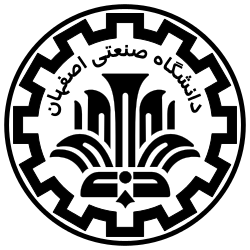
\includegraphics[width=.2\textwidth]{iut}\\
    گزارش تکلیف پیاده\ سازی الگوریتم\\
    \lr{Back Propagation}
}
\author{داریوش حسن\ پور آده}
\date{۹۳۰۸۱۶۴}
\maketitle
\قسمت{مقدمه}
در این تکلیف هدف درک عمیق\ تر الگوریتم \بپ\فوتنت{Back Propagation} از طریق پیاده\ سازی آن و اعمال الگوریتم پیاده\ سازی شده برای تشخیص اعداد دست\ نویس مجموعه داده\ ی \منست می\ باشد. داده\ های آموزشی \منست شامل ۶۰,۰۰۰ قطعه عکس از اعداد دست\ نویس برچسب خورده می\ باشد. ترکیبی که برای آموزش شبکه\ ی عصبی در نظر گرفته شده است، ساختار ۳ لایه\ ای
$784{\times}100{\times}10$
برای یادگیری در نظر گرفته شده است که دارای ۷۸۴ عدد داده\ ی ورودی و ۱۰۰ نورون در لایه\ ی مخفی و ۱۰ نورون در لایه\ ی خروجی شبکه می\ باشد.
\قسمت{برنامه\ ی نوشته شده}
برنامه به زبان \lr{C++} در محیط لینوکس نوشته شده است، که داده\ های آموزشی و تست ذخیره شده به فرمت متلب را از پوشه\ ی داده\ ها می\ خواند. برای راحتی کار ابتدا داده\ های \منست را به در متلب بارگذاری کردم و سپس با توجه به اندیس\ های داده\ های ارزیاب\فوتنت{Evaluation Set} داده\ های اولیه را به دو دسته\ ی داده\ های آموزشی و داده\ های ارزیابی تقسیم کرده و سپس داده\ های ارزیابی را به انتهای داده\ های آموزشی اضافه کرده و در نهایت داده\ ها را در یک فایل به فرمت متلب ذخیره سازی کردم. از آنجایی که داده\ های ارزیابی در انتهای داده\ های آموزشی اضافه شده\ اند داده\ های آموزشی که تعدادشان ۵۰,۰۰۰ عدد و داده\ های ارزیابی به تعداد ۱۰,۰۰۰ عدد به راحتی قابل جداسازی می\ باشد. برای داده\ های تست نیز همین روند اجرا می\ شود، یعنی داده\ ها در متلب بارگذاری می\ شود و سپس در فایلی ذخیره می\ شود.\بند
بعد از آماده و ذخیره\ سازی داده\ های آموزشی و تست، داده\ های ذخیره شده به فرمت متلب از فایل\ های مربوطه خوانده می\ شود و بعد از نگاشت ساختمان داده\ ی داده\ های خوانده شده به ساختمان داده\ ای که برنامه\ ی نوشته شده با آن سازگار می\ باشد شبکه\ ی عصبی با ساختار گفته شده در قسمت قبل ساخته شده و مقدار دهی\ اولیه می\ شود. سپس داده\ های آموزشی بسته به نوع آموزش دسته\ ای\فوتنت{Batch} یا برخط\فوتنت{Online} به ازای هریک از قسمت\ های آمده در تکلیف آموزش، ارزیابی و تست می\ گردد. در مورد قطع زود هنگام آموزش، آموزش شبکه در ۲ صورت زودتر از موعد مقرر(حداکثر تعداد دوره\فوتنت{Epoch}) قطع می\ شود. اولی در صورتی که بیش از ۵ دوره پشت سرهم درصد دقت شبکه بروی داده\ های ارزیابی کاهش پیدا کند؛ و دومی در صورتی که میانگین مقادیر \lr{MSE} خروجی\ های شبکه در داده\ های ارزیابی کمتر از ۰.۰۱ شود.\بند
\زیرقسمت{وابستگی\ های برنامه}
در مورد وابستگی\ های\فوتنت{Dependency} برنامه\ ی نوشته شده، برنامه از کتابخانه\ ی معروف \lr{Boost} نسخه\ ی ۱.۵۴ برای استفاده\ های عمومی و از کتابخانه\ ی \lr{Matio} نسخه\ ی ۱.۵.۲ برای بارگذاری داده\ های  ذخیره شده به فرمت متلب استفاده می\ شود. از آنجایی که برای آموزش شبکه\ های عصبی عملیات مبتنی بر ماتریس\ ها ساده\ ترین راه برای پیاده\ سازی می\ باشد از کتابخانه\ ی \lr{Eigen} نسخه\ ی ۳.۲.۷ برای کاربردهای ماتریسی و جبرخطی استفاده شده است. دو کتابخانه\ ی اول باید در سیستم\ عامل نصب و قابل دسترسی برای کامپیالر باشد ولی در مورد کتابخانه\ ی سوم به صورت جاسازی\ شده\فوتنت{Embedded} همراه کدها آمده است. برنامه توسط کامپایلر \lr{g++} نسخه\ ی ۴.۸.۴ کامپایل شده و نیز برای راحتی کامپایل کردن برنامه از ابزار \lr{CMake} نسخه\ ی ۲.۸.۱۲.۲ استفاده شده است که هردوی این\ ها باید در سیستم نصب باشد. همچنین جهت مدیریت نخسه\ ی برنامه\فوتنت{Control Version} از ابزار \lr{Git} نسخه\ ی ۲.۶.۳ استفاده شده است، که البته داشتن ابزار \تاکید{مدیریت نسخه} برای کامپایل برنامه مورد نیاز نیست و صرفا جهت توسعه\ ی برنامه مورد استفاده قرار گرفته است.
\newpage
\قسمت{نتایج قسمت\ ها}
\زیرقسمت{قسمت الف}
در این قسمت ما با در نظر گرفتن مقدار گام ۰.۴ به تعداد حداکثر ۳۰ دوره داده\ های آموزشی را به شبکه به صورت دسته\ ای خوراندیم، و در نهایت دقت ۵۹.۵۱٪ را رو داده\ های تست بدست آوردیم. توجه شود که این مقدار از آنچه که در کتاب آمده کمتر است زیرا اول اینکه در کتاب داده\ ها به صورت دسته\ های کوچک\فوتنت{Mini-Batch} با اندازه\ های ۱۰ به شبکه خورانده است پس در نتیجه سریع\ تر به مقدار هدف همگرا شده است. دوم اینکه همان\ طور که میدانیم آموزش داده\ ها به صورت دسته\ ای باعث می\ شود که شبکه با ملایمت\فوتنت{Smooth} بیشتری به سمت کمینه\ ی محلی پیش برود بنابرین برای اینکه این شبکه دقت بالایی برسد باید تعداد دوره\ ی بیشتری آموزش می\ دید\زیرنویس{برای آموزش به صورت دسته\ ای که به دقت ۵۹٪ برسد، نزدیک به ۶ ساعت آموزش نیاز داشت!!}.
نمودار دقت بروی داده\ های ازریابی در طی آموزش در شکل
\ref{fig:section_a_batch_acc}
آمده است. که دقت بروی داده\ های ارزیابی از ۱۲.۱۳٪ شروع شده و در نهایت بعد از ۳۰ دوره به دقت ۵۸.۶۴٪ رسیده است؛ همان\ طور که در شکل
\ref{fig:section_a_batch_acc}
نیز مشاهده می\ کنیم دقت به صورت ملایم افزایش یافته و افت\ وخیزی در میزان دقت در هر دوره مشاهده نمی\ شود(برعکس آنچه که در آموزش به شیوه\ ی برخط مشاهده می\ شود).\بند
\begin{figure}[h!]
\centering
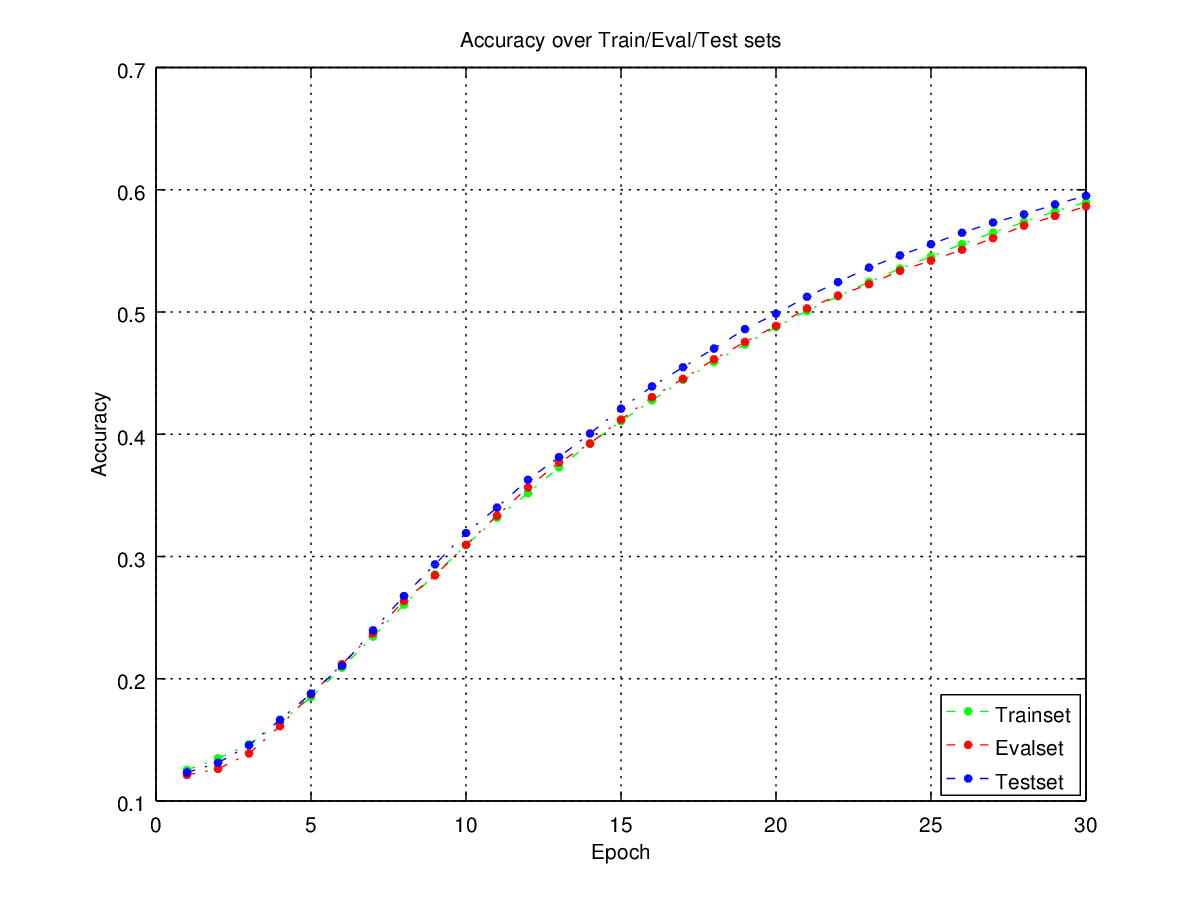
\includegraphics[width=\textwidth]{1_batch_acc}
\caption{مقدار دقت بروی داده\ های آموزشی، ارزیاب و تست در دوره\ های مختلف برای قسمت الف}\label{fig:section_a_batch_acc}
\end{figure}
نمودار مقادیر \مسی خروجی\ های شبکه در داده\ های آموزشی، ارزیاب و تست در شکل
\ref{fig:section_a_batch_mse}
آمده است. همان\ طور که مشاهده می\ شود مقادیر \مسی کلیه\ ی خروجی\ ها تقریبا با یک روند یکنواخت در طی دوره\ های مختلف کاهش پیدا می\ کند\زیرنویس{جدول مقادیر \مسی خروجی\ ها همراه کدها\ ی برنامه آمده است.}.
\begin{figure}[h!]
\centering
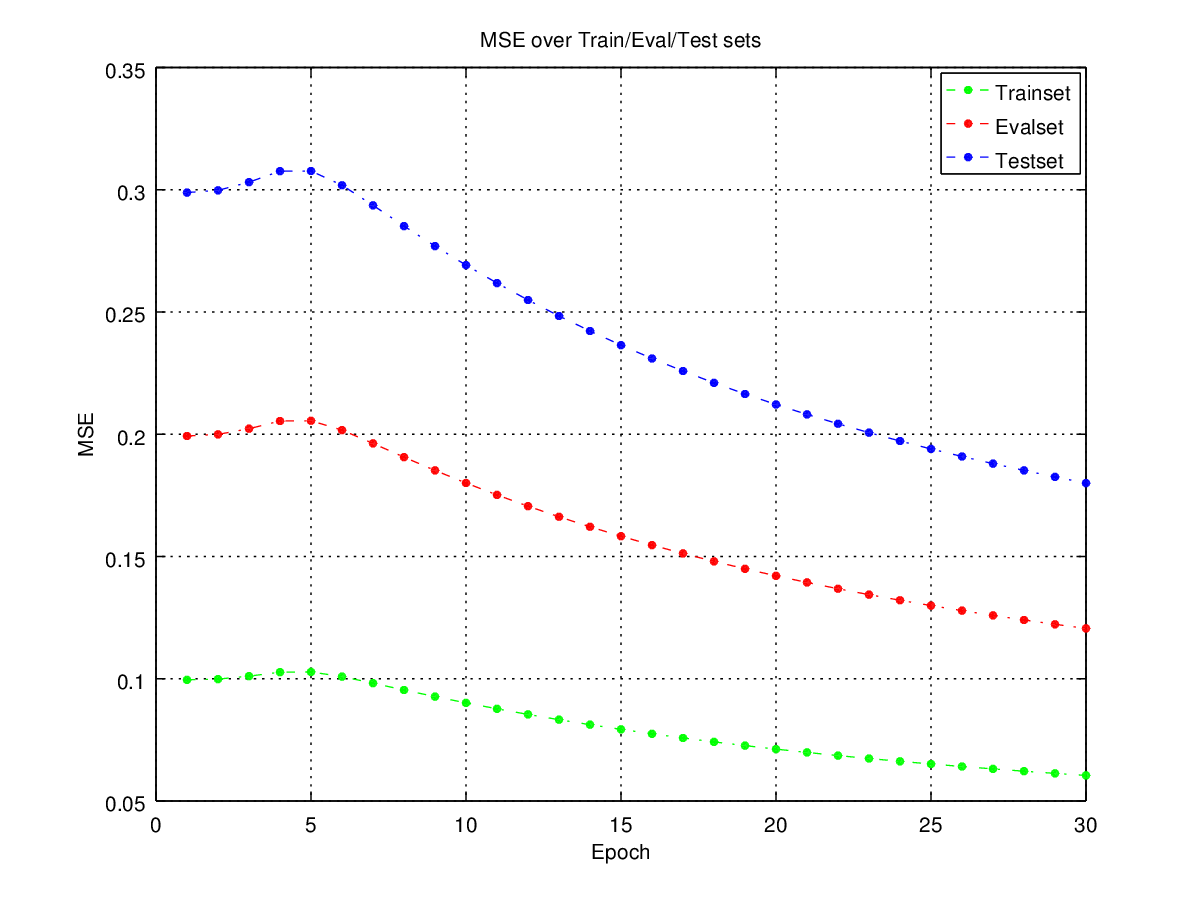
\includegraphics[width=\textwidth]{1_batch_mse}
\caption{مقدار میانگین \مسی خروجی\ های شبکه بروی داده\ های آموزشی، ارزیاب و تست در دوره\ های مختلف برای قسمت الف}\label{fig:section_a_batch_mse}
\end{figure}
\قسمت{قسمت ب}
در این قسمت با در نظر گرفتن مقدار گام ۰.۳ به صورت برخط به آموزش داده\ ها پرداختیم که در نهایت به دقت ۹۶.۳۵٪ با حداکثر تعداد ۳۰ دوره بروی داده\ های تست رسیدیم که اختلاف زیادی با آنچه که در قسمت اول مشاهده کردیم دارد. نمودار دقت و میزان \مسی در شکل\ های
\ref{fig:section_b_online_acc} و \ref{fig:section_b_online_mse}
آمده\ اند. در صورت مقایسه\ ی شکل
\ref{fig:section_b_online_acc}
با شکل
\ref{fig:section_a_batch_acc}
به وضوح مشاهده می\ شود که دقت در یادگیری برخط افت\ وخیز زیادی نسبت به یادگیری دسته\ ای دارد ولی در تعداد دوره\ ی یکسان دقت بالایی نسبت به یادگیری دسته\ ای دارد. همچنین با مقایسه\ ی شکل
\ref{fig:section_b_online_mse} و \ref{fig:section_a_batch_mse}
مشاهده می\ شود که برخلاف یادگیری دسته\ ای که مقادیر \مسی خروجی\ های آن یک\ نواخت کاهش می\ یابد ولی در یادگیری برخط مقادیر \مسی افت\ و\ خیز زیادی دارد.\بند
بااینکه دقت یادگیری به روش برخط بهتر از یادیگری به روش دسته\ ای می\ باشد ولی این روش همانند روش یادگیری دسته\ ای هیچ\ یک از معیارها توقف زود هنگام گفته شده در قسمت\ های گذشته را ارضا نکرده و بعد از گذران حداکثر تعداد دوره(۳۰ عدد) به پایان مهلت یادگیری خود رسیده است.
\begin{figure}
\centering
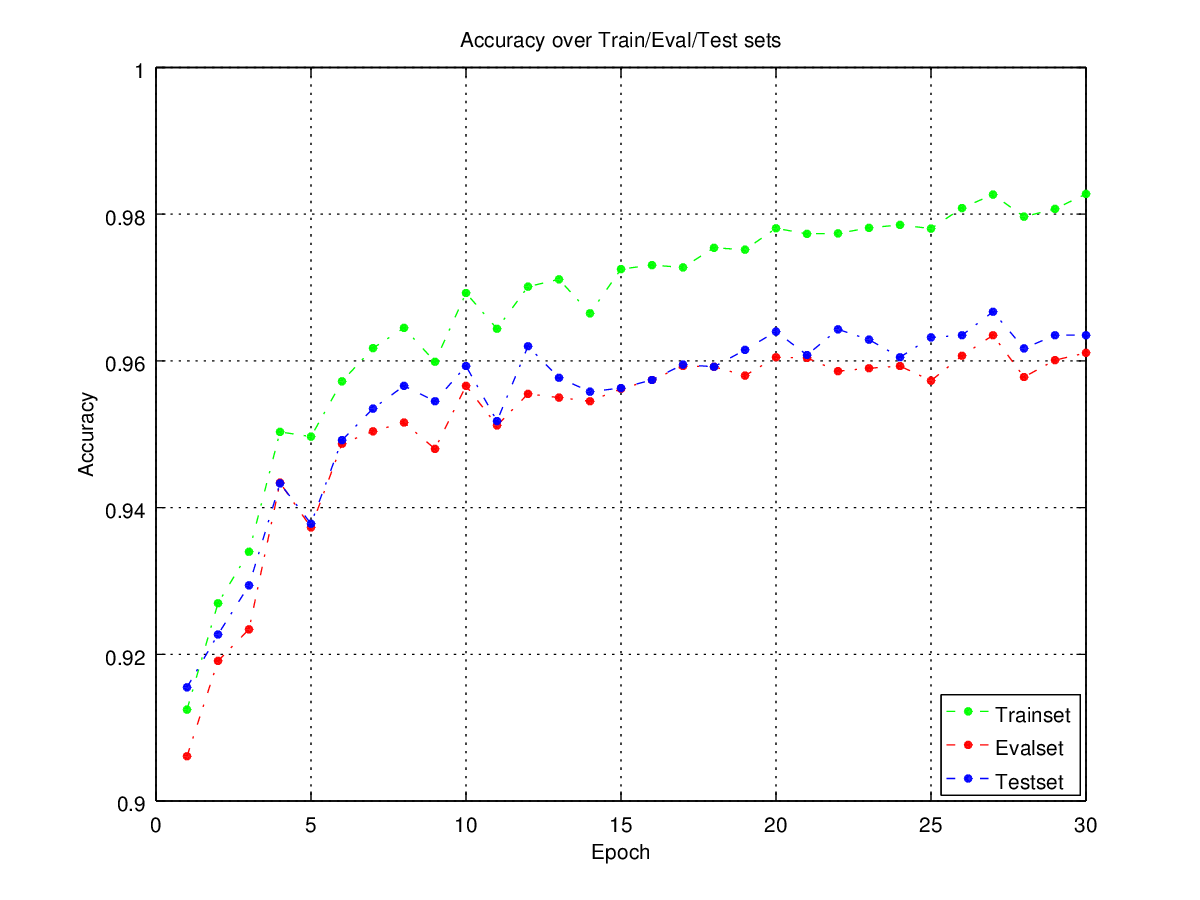
\includegraphics[width=.9\textwidth]{2_online_acc}
\caption{مقدار دقت بروی داده\ های آموزشی، ارزیاب و تست در دوره\ های مختلف برای قسمت ب}\label{fig:section_b_online_acc}
\end{figure}
\begin{figure}
\centering
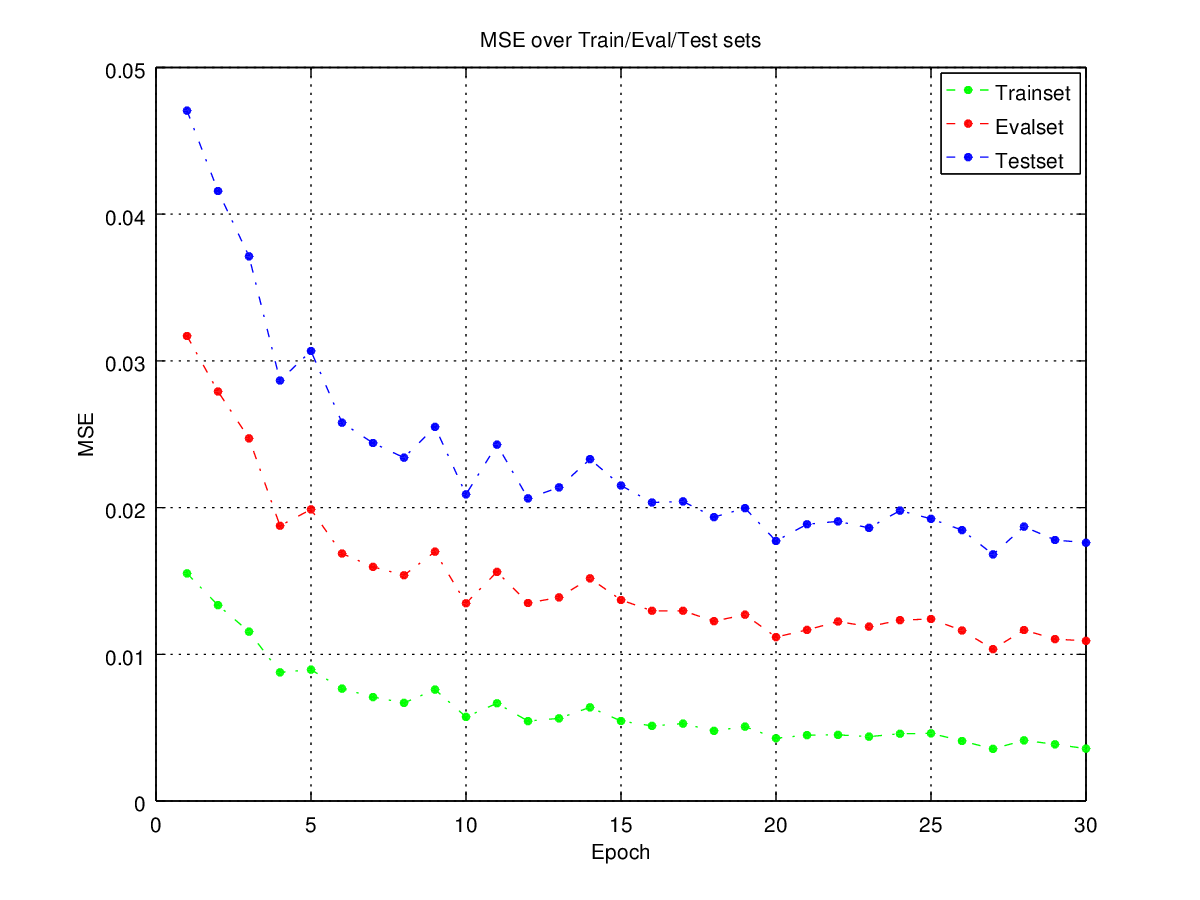
\includegraphics[width=.9\textwidth]{2_online_mse}
\caption{مقدار میانگین \مسی خروجی\ های شبکه بروی داده\ های آموزشی، ارزیاب و تست در دوره\ های مختلف برای قسمت ب}\label{fig:section_b_online_mse}
\end{figure}
برای مقایسه\ ی اثر یادگیری برخط اختلاف دقت و مقادیر \مسی بدست آمده\ ی قسمت الف را با این قسمت بدست آورده که در شکل\ های
\ref{fig:section_b_online_diff_acc} و \ref{fig:section_b_online_diff_mse}
آمده است. همان\ طور که در شکل
\ref{fig:section_b_online_diff_acc}
مشاهده می\ شود در کلیه\ ی دوره\ ها میزان دقت شبکه\ ای که به صورت برخط یادگرفته بیشتر بصورت چشم گیری بیشتر از دقت شبکه\ ای است که با یادگیری دسته\ ای آموزش دیده است ولی به مرور زمان یادگیری دسته\ ای به صورت یکنواخت اختلاف دقتش را با یادگیری برخط کاهش داده ولی در یک طول دوره\ ی یکسان یادگیری برخط بوضوح دقت بهتری را ارائه داده است. همچنین در مورد اختلاف مقادیر \مسی همیشه یادگیری برخط مقدار \مسی کمتری نسبت به یادگیری دسته\ ای داشته ولی به مرور زمان همزمان با افزایش دقت یادگیری دسته\ ای میزان اختلاف \مسی کاهش یافته است.\بند
ولی از طرف دیگر زمان یادگیری، یادگیری برخط تقریبا ۲ برابر یادگیری دسته\ ای می\ باشد\زیرنویس{تقریبا زمان یادگیری برخط به ازای ۳۰ دوره نزدیک به ۱۵ ساعت شد!!} و علت این امر این است که به ازای هر داده\ ی آموزشی(۵۰,۰۰۰ عدد) یک بار باید تمامی وزن\ های شبکه(به تعداد ۷۸۴,۰۰۰ عدد) بروزرسانی شود که به ازای یک دوره تقریبا
\lr{$3.92e+10$} 
وزن بروزرسانی شده است در حالی که در یادگیری دسته\ ای در هر دوره فقط ۷۸۴,۰۰۰ وزن بروز رسانی شده است و این یعنی
$1 \over 50,000$
برابر بروزرسانی کمتر!!
\newpage
\begin{figure}[h!]
\centering
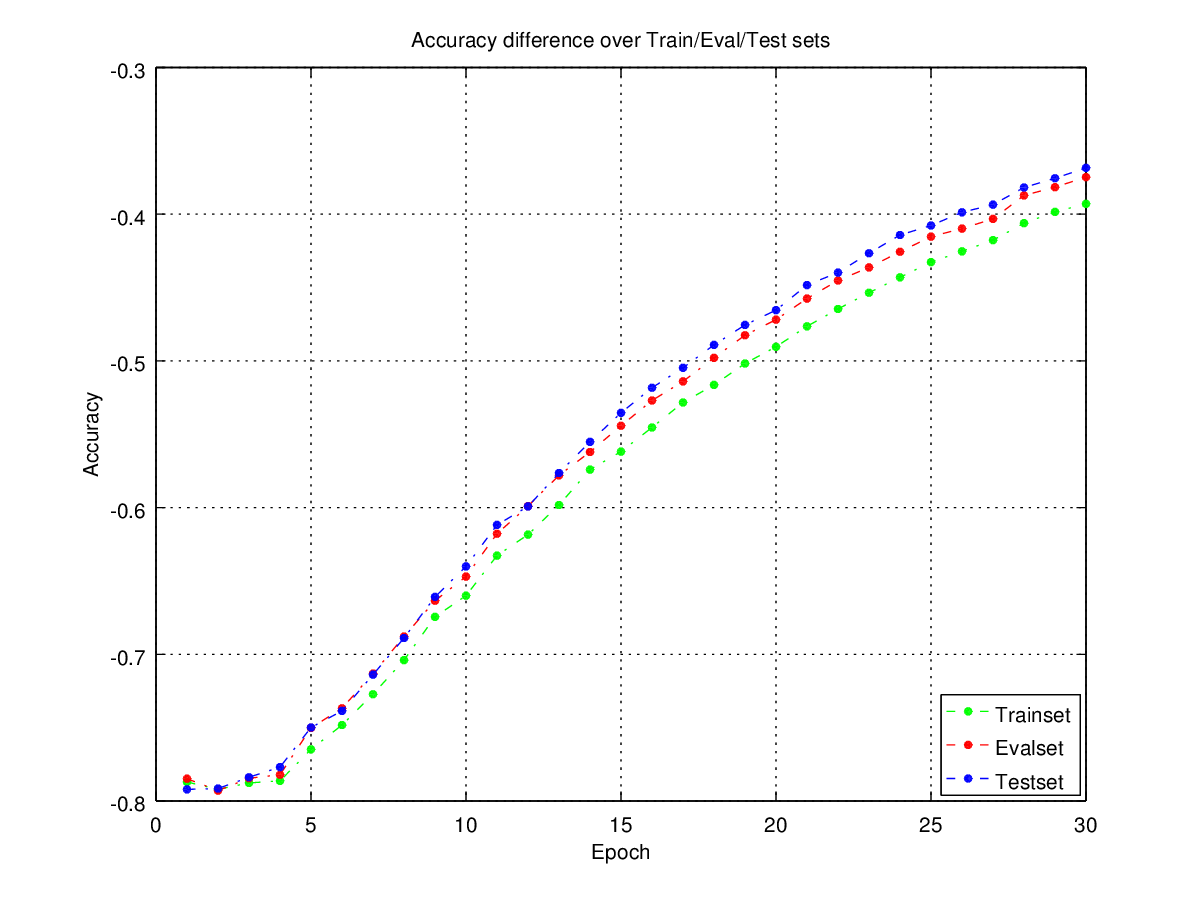
\includegraphics[width=.9\textwidth]{2_online_diff_acc}
\caption{مقدار اختلاف دقت قسمت الف و قسمت ب بروی داده\ های آموزشی، ارزیاب و تست در دوره\ های مختلف}\label{fig:section_b_online_diff_acc}
\end{figure}
\begin{figure}[h!]
\centering
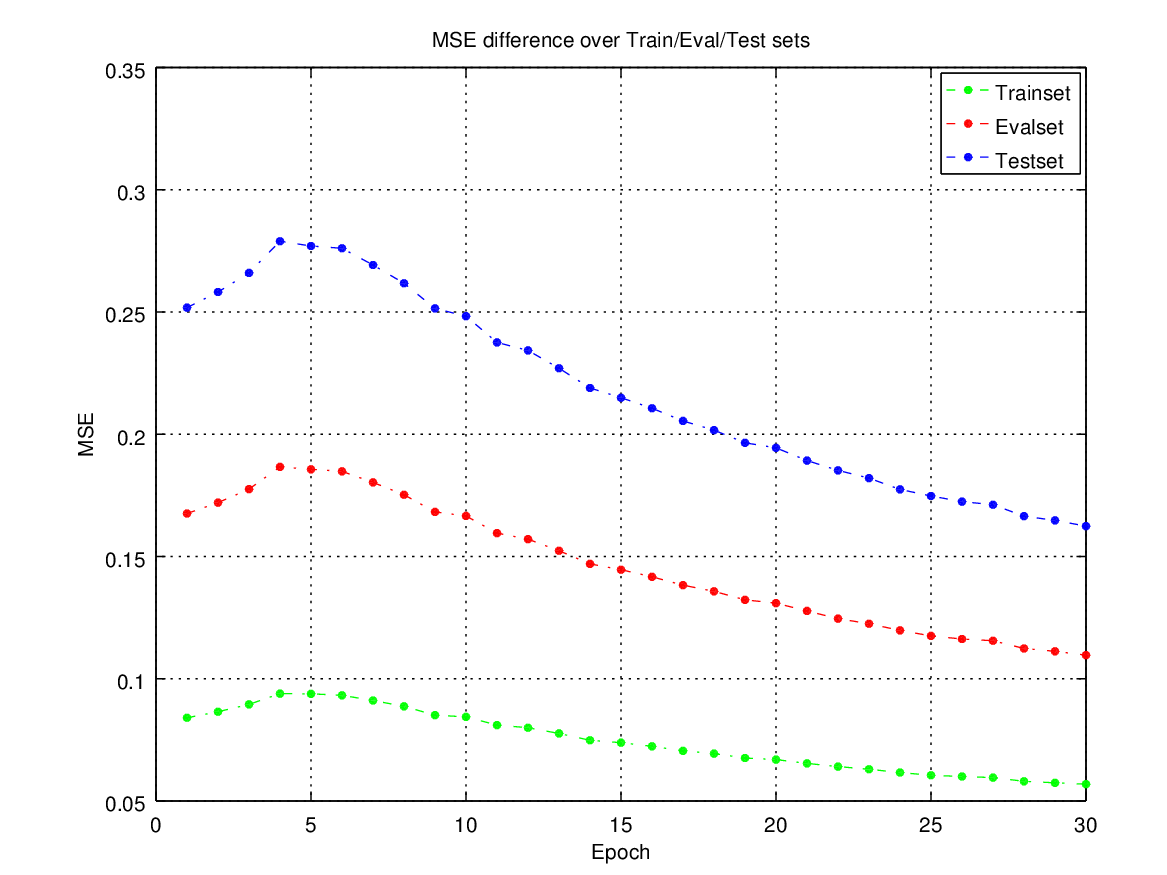
\includegraphics[width=.9\textwidth]{2_online_diff_mse}
\caption{مقدار اختلاف مقادیر \مسی قسمت الف و قسمت ب بروی داده\ های آموزشی، ارزیاب و تست در دوره\ های مختلف}\label{fig:section_b_online_diff_mse}
\end{figure}
\قسمت{قسمت ج}
در این قسمت با در نظر گرفتن مقدار مومنتم ۰.۲ و مقدار گام ۰.۴(مثل قسمت الف) به صورت دسته\ ای داده\ های آموزشی را به شبکه دادیم دقت این قسمت بروی داده\ های تست ۵۴.۳٪ می\ باشد که مقدار دقت کمتر از آنچه که در الف بدست آمده است دارا می\ باشد، که چون در این قسمت نیز از نحوه\ ی آموزش دسته\ ای استفاده شده، علت پایین بودن نسبی دقت در این قسمت مشابه قسمت الف می\ باشد. همچنین مشابه قسمت الف شبکه را بعد از هر دوره با داده\ های ارزیابی آزمودیم که میزان دقت و مقادیر \مسی خروجی\ های آن در شکل\ های
\ref{fig:section_c_mom_acc} و \ref{fig:section_c_mom_mse}
آمده است.\بند
برای مقایسه\ ی اثر استفاده\ ی مومنتم در قسمت الف تکلیف اختلاف دقت و مقادیر \مسی بدست آمده\ ی قسمت الف را با این قسمت بدست آورده که در شکل\ های
\ref{fig:section_c_mom_diff_acc} و \ref{fig:section_c_mom_diff_mse}
آمده است. همان\ طور که در شکل
\ref{fig:section_c_mom_diff_acc}
مشاهده می\ شود در ۵-۶ دوره\ ی اول میزان دقت بدست آمده در آموزش با استفاده از مومنتم بیشتر از آموزش بدون استفاده از مومنتم می\ باشد ولی بعد ازچند دوره دقت شبکه\ ای که از مومنتم استفاده نکرده است(قسمت الف) بیشتر است -- که این بخاطر خاصیت اینرسی\ ای است که روش مومنتم دارد و باعث می\ شود وزن در مقابل تغییرات دروه\ ای مقاومت بیشتری از خود نشان دهند.
\newpage
\begin{figure}[h!]
\centering
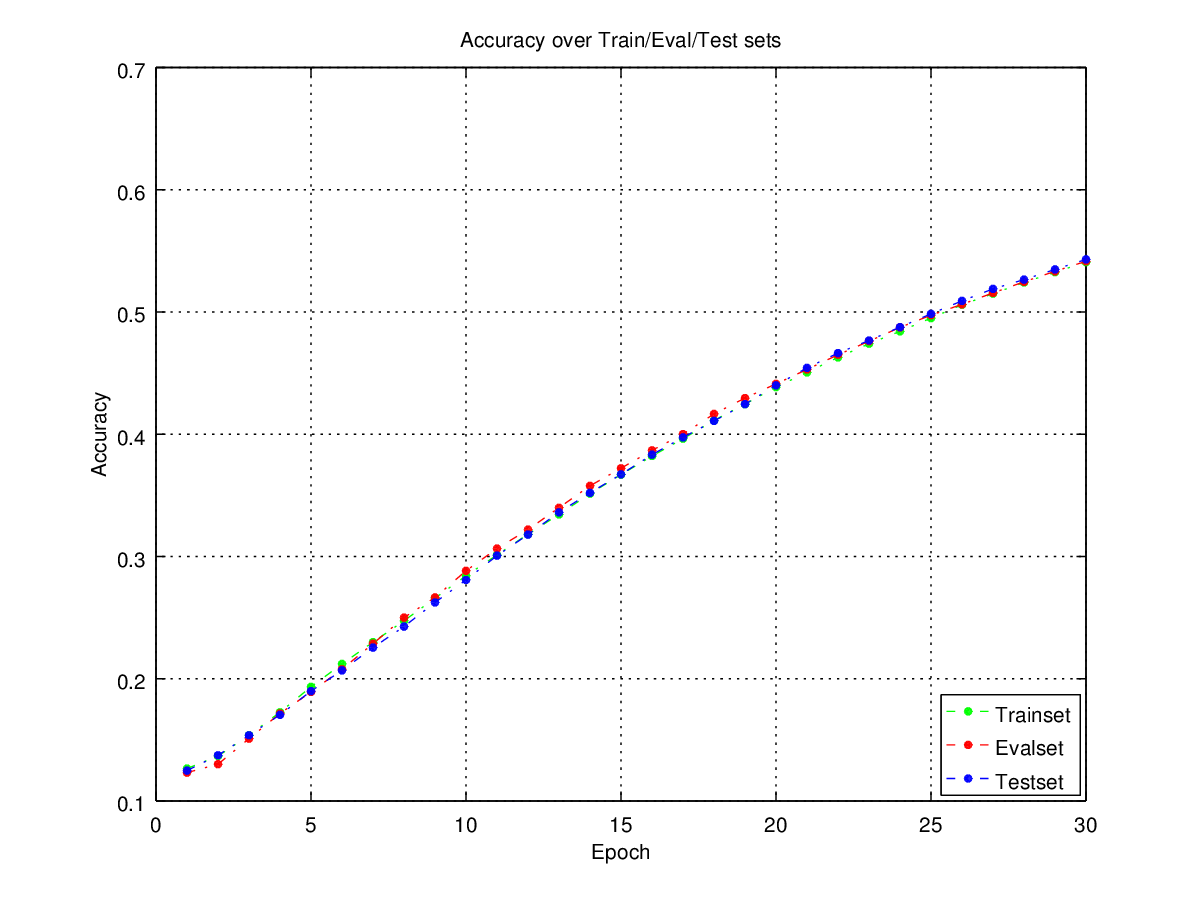
\includegraphics[width=.9\textwidth]{3_mom_acc}
\caption{مقدار دقت بروی داده\ های آموزشی، ارزیاب و تست در دوره\ های مختلف برای قسمت ج}\label{fig:section_c_mom_acc}
\end{figure}
\begin{figure}[h!]
\centering
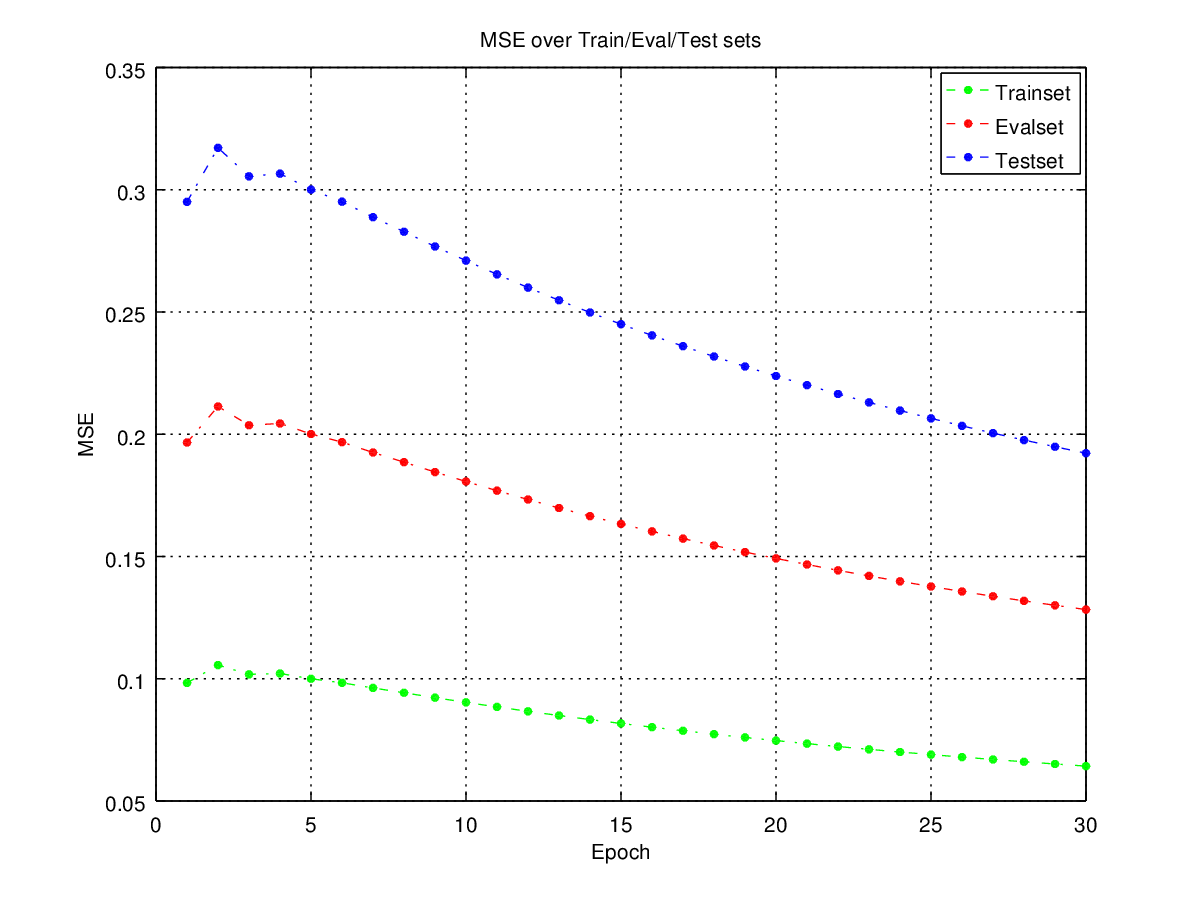
\includegraphics[width=.9\textwidth]{3_mom_mse}
\caption{مقدار میانگین \مسی خروجی\ های شبکه بروی داده\ های آموزشی، ارزیاب و تست در دوره\ های مختلف برای قسمت ج}\label{fig:section_c_mom_mse}
\end{figure}
\begin{figure}[h!]
\centering
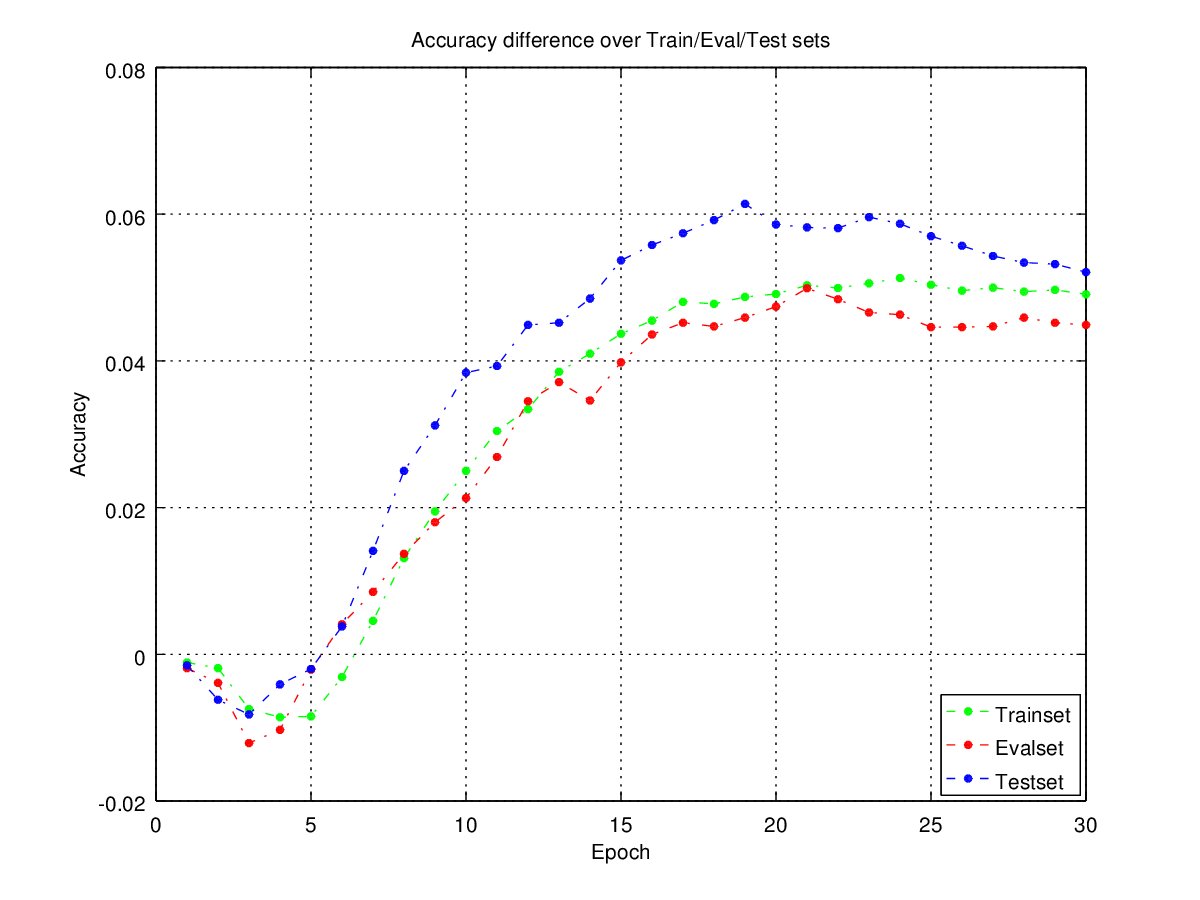
\includegraphics[width=.9\textwidth]{3_mom_diff_acc}
\caption{مقدار اختلاف دقت قسمت الف و قسمت ج بروی داده\ های آموزشی، ارزیاب و تست در دوره\ های مختلف}\label{fig:section_c_mom_diff_acc}
\end{figure}
\begin{figure}[h!]
\centering
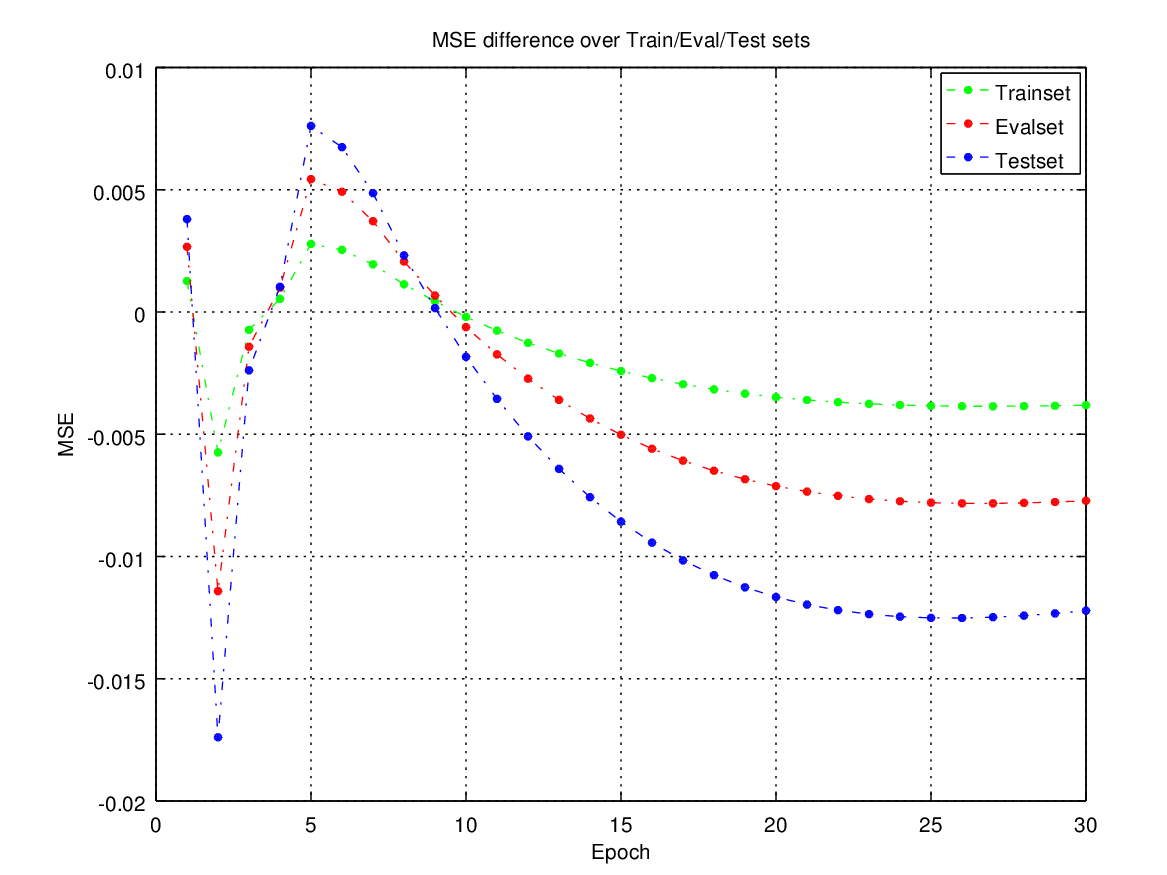
\includegraphics[width=.9\textwidth]{3_mom_diff_mse}
\caption{مقدار اختلاف مقادیر \مسی قسمت الف و قسمت ج بروی داده\ های آموزشی، ارزیاب و تست در دوره\ های مختلف}\label{fig:section_c_mom_diff_mse}
\end{figure}
\newpage
\قسمت{قسمت د}
در این قسمت با در نظر گرفتن مقدار منتظم\ سازی\فوتنت{Regularization} برابر با ۰.۱ و مقدار گام ۰.۴(مثل قسمت الف) به صورت دسته\ ای داده\ های آموزشی را به شبکه دادیم دقت این قسمت بروی داده\ های تست ۶۲.۷۶٪ می\ باشد که از دقت نهایی قسمت الف به میزان چند درصدی بیشتر است، که چون در این قسمت نیز از نحوه\ ی آموزش دسته\ ای استفاده شده، علت پایین بودن نسبی دقت در این قسمت مشابه قسمت الف می\ باشد. همچنین مشابه قسمت الف شبکه را بعد از هر دوره با داده\ های ارزیابی آزمودیم که میزان دقت و مقادیر \مسی خروجی\ های آن در شکل\ های
\ref{fig:section_d_reg_acc} و \ref{fig:section_d_reg_mse}
آمده است.
\newpage
\begin{figure}
\centering
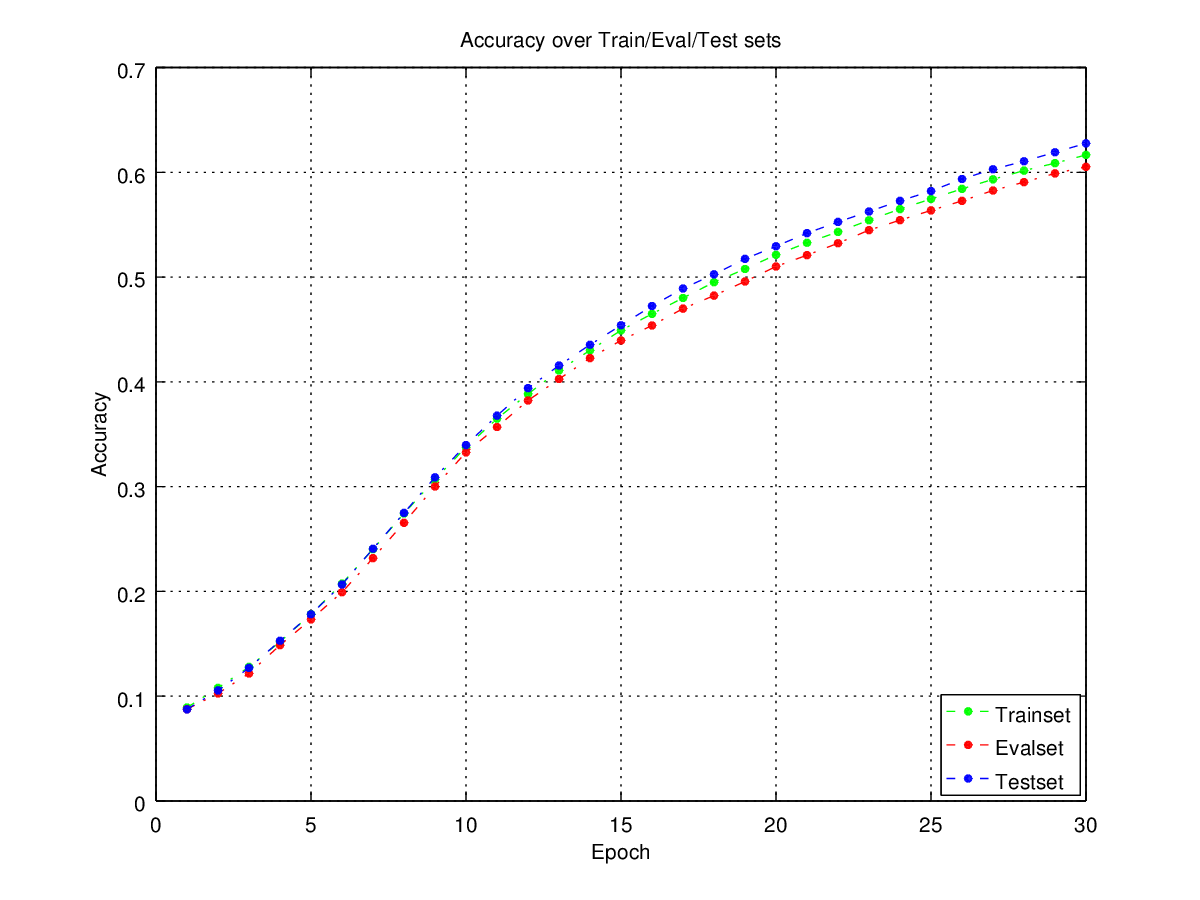
\includegraphics[width=.9\textwidth]{4_reg_acc}
\caption{مقدار دقت بروی داده\ های آموزشی، ارزیاب و تست در دوره\ های مختلف برای قسمت ج}\label{fig:section_d_reg_acc}
\end{figure}
\begin{figure}
\centering
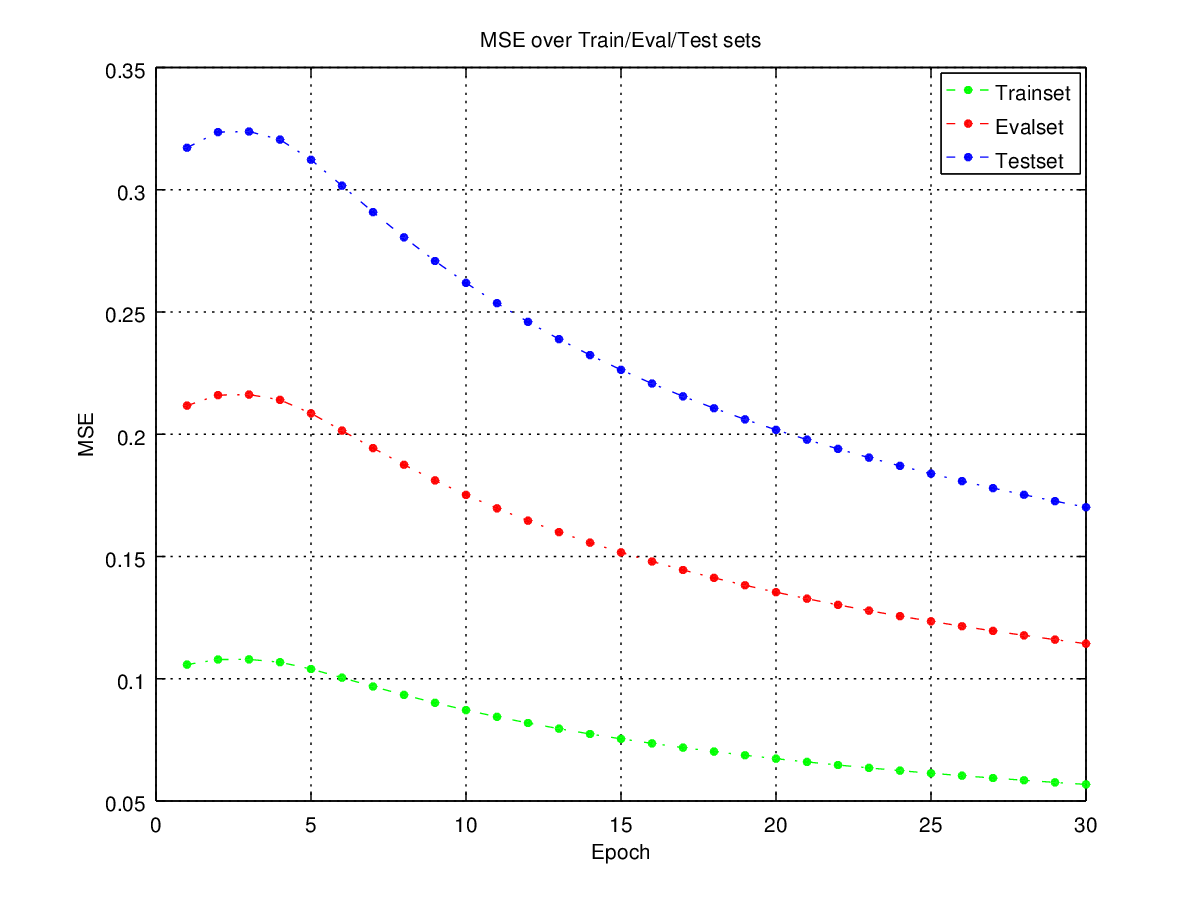
\includegraphics[width=.9\textwidth]{4_reg_mse}
\caption{مقدار میانگین \مسی خروجی\ های شبکه بروی داده\ های آموزشی، ارزیاب و تست در دوره\ های مختلف برای قسمت ج}\label{fig:section_d_reg_mse}
\end{figure}
برای مقایسه\ ی اثر استفاده\ ی منتظم\ سازی در قسمت الف تکلیف اختلاف دقت و مقادیر \مسی بدست آمده\ ی قسمت الف را با این قسمت بدست آورده که در شکل\ های
\ref{fig:section_d_reg_diff_acc} و \ref{fig:section_d_reg_diff_mse}
آمده است. همان\ طور که در شکل
\ref{fig:section_d_reg_diff_acc}
مشاهده می\ شود در ابتدای کار(۱۲-۱۵ دوره\ ی اول) میزان دقت قسمت الف بیشتر بوده ولی بعد از این قسمت دقت قسمت د چند درصدی بیشتر از قسمت الف می\ شود(همین مساله برای اختلاف مقادیر \مسی نیز برقرار است).

\begin{figure}
\centering
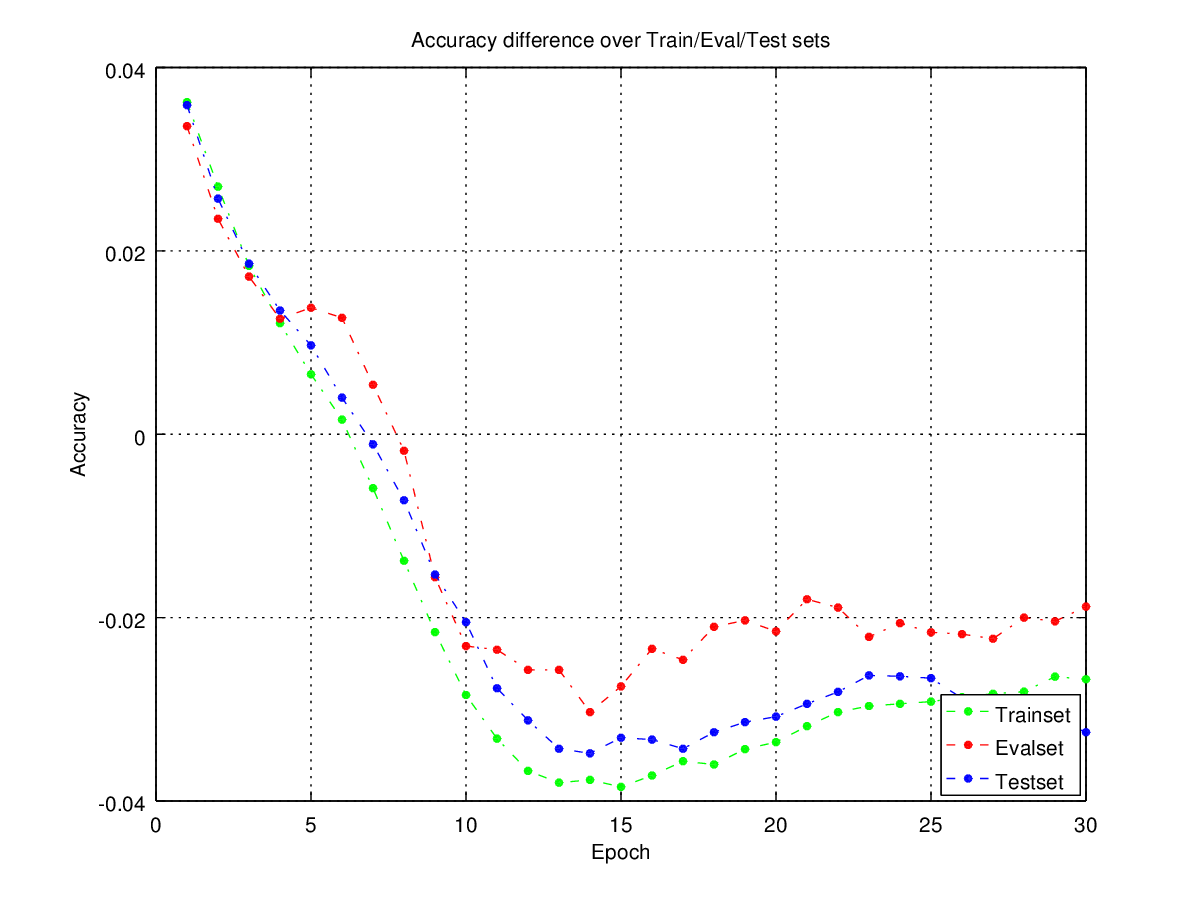
\includegraphics[width=.9\textwidth]{4_reg_diff_acc}
\caption{مقدار اختلاف دقت قسمت الف و قسمت د بروی داده\ های آموزشی، ارزیاب و تست در دوره\ های مختلف}\label{fig:section_d_reg_diff_acc}
\end{figure}
\begin{figure}
\centering
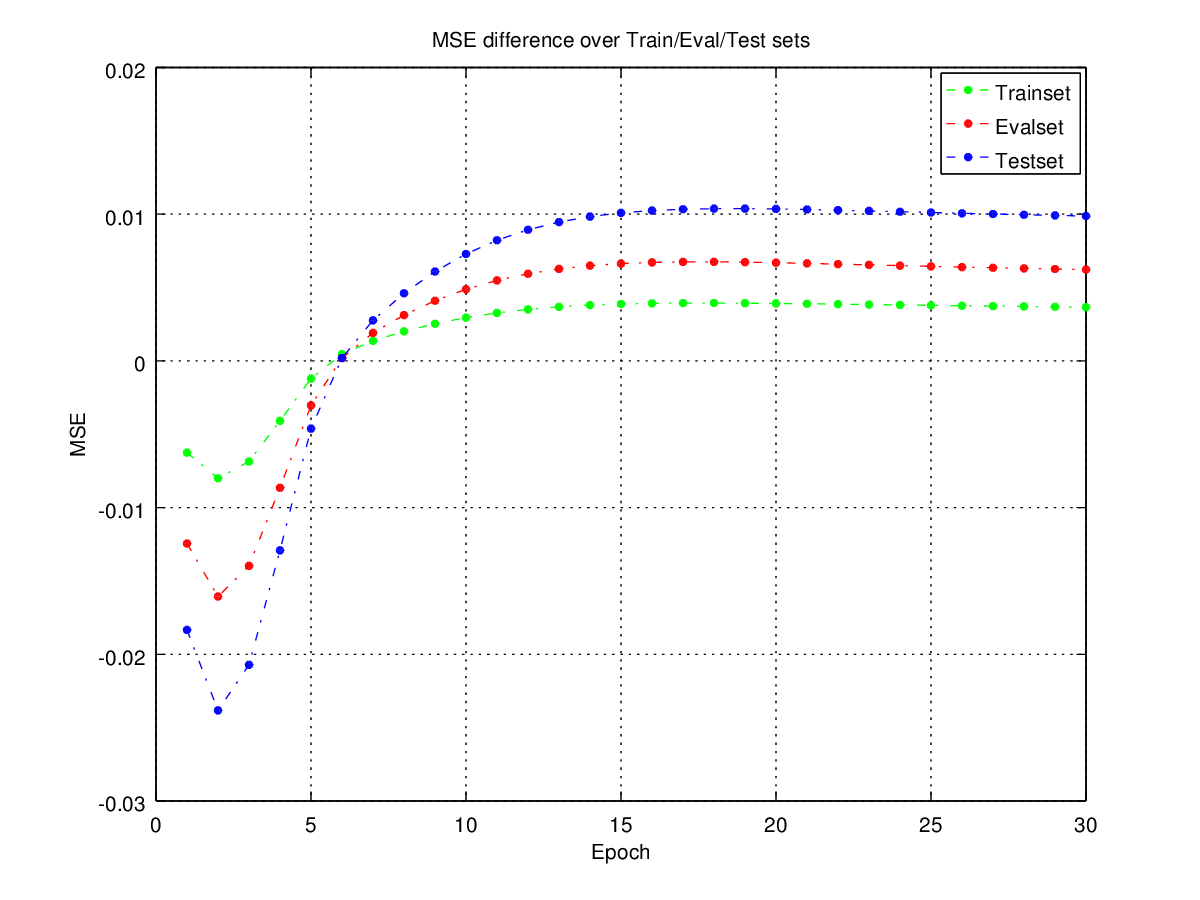
\includegraphics[width=.9\textwidth]{4_reg_diff_mse}
\caption{مقدار اختلاف مقادیر \مسی قسمت الف و قسمت د بروی داده\ های آموزشی، ارزیاب و تست در دوره\ های مختلف}\label{fig:section_d_reg_diff_mse}
\end{figure}
\قسمت{قسمت آخر(نمره اضافی)}
بنده بروی داده\ های ورودی(داده\ های مربوط عکس\ های -- نه برچسب\ ها) عملیات کاهش بعد \lr{PCA} زدم ابعاد داده\ های عکس ها را از ۷۸۴ بعد به ۱۰۰ بعد کاهش دادم و سپس با شبکه\ ای با ساختار
$100 \times 100 \times 10$
داده\ ها را آموزش دادم. در این حالت چون تعداد ورودی\ های شبکه کاهش یافته می\ توان با تعداد نورون کمتری در لایه\ ی مخفی الگوی داده\ ها را پوشش داد؛ که این کاهش بعد به کاهش حجم محاسباتی و بروزرسانی وزن می\ انجامد. این کاهش در ساختار این شبکه حدود ۸۷٪‌ از حجم محاسباتی\ ای که در شبکه\ ای که داده\ های اولیه را یاد می\ گرفت، صرف\ جویی شده که در نهایت موجود می\ شود در یک زمان محدود تعداد دوره\ ی بیشتری نسبت به شبکه\ ی پیشین طی کند و با در نظر گرفتن زمان یکسان دقت بیشتری بدست آورد. همچنین این کاهش بعد حدود ۸۳٪ از حجم حافظه\ ی مورد نیاز در مرحله قبل را نیز صرفه\ جویی کرده است.\بند
در آموزش این قسمت از روش دسته\ های کوچک\فوتنت{Mini-Batch} با اندازه\ های ۱۰تایی استفاده کردم که دقت و سرعت همگرایی را نسبت کلیه\ ی قسمت\ های فوق را بیشتر کرد و میزان دقت آن بروی داده\ های تست ۹۶.۷۹٪ بدست آمد. همان\ طور که قبلا گفته شد کاهش سایز داده\ ها به کاهش وزن\ های شبکه کمک می\ کند و همچنین استفاده از روش دسته\ های کوچک بجای روش\ های یادگیری دسته\ ای و برخطی به میزان سرعت یادگیری و ملایم بودن دقت شبکه کمک میکند به\ طوری که آموزش قسمت الف که به دقتی در حدود ۵۹٪ برسد نزدیک ۶ ساعت زمان برد و در قسمت ب نیز برای اینکه به دقتی در حدود ۹۶.۳۵٪ داشت، به ۱۵ ساعت آموزش  و ۳۰ دوره نیاز داشت در حالی که بعد از کاهش بعد و استفاده از روش یادگیری دسته\ های کوچک بعد از ۷ دوره که فقط در ۱۰ دقیقه انجام شد میزان میانگین مقادیر \مسی به زیر ۰.۰۱ و دقت ۹۶.۷۹٪ را داشت که هم در زمان و هم در تعداد دوره\ ها و هم در دقت از کلیه\ ی نتایج قسمت\ های قبلی برتریت داشت. میزان دقت و مقادیر \مسی شبکه بعد از استخراج ویژگی\ ها در اشکال
\ref{fig:section_e_pca_acc} و \ref{fig:section_e_pca_mse}
آمده است.
\begin{figure}[t!]
\centering
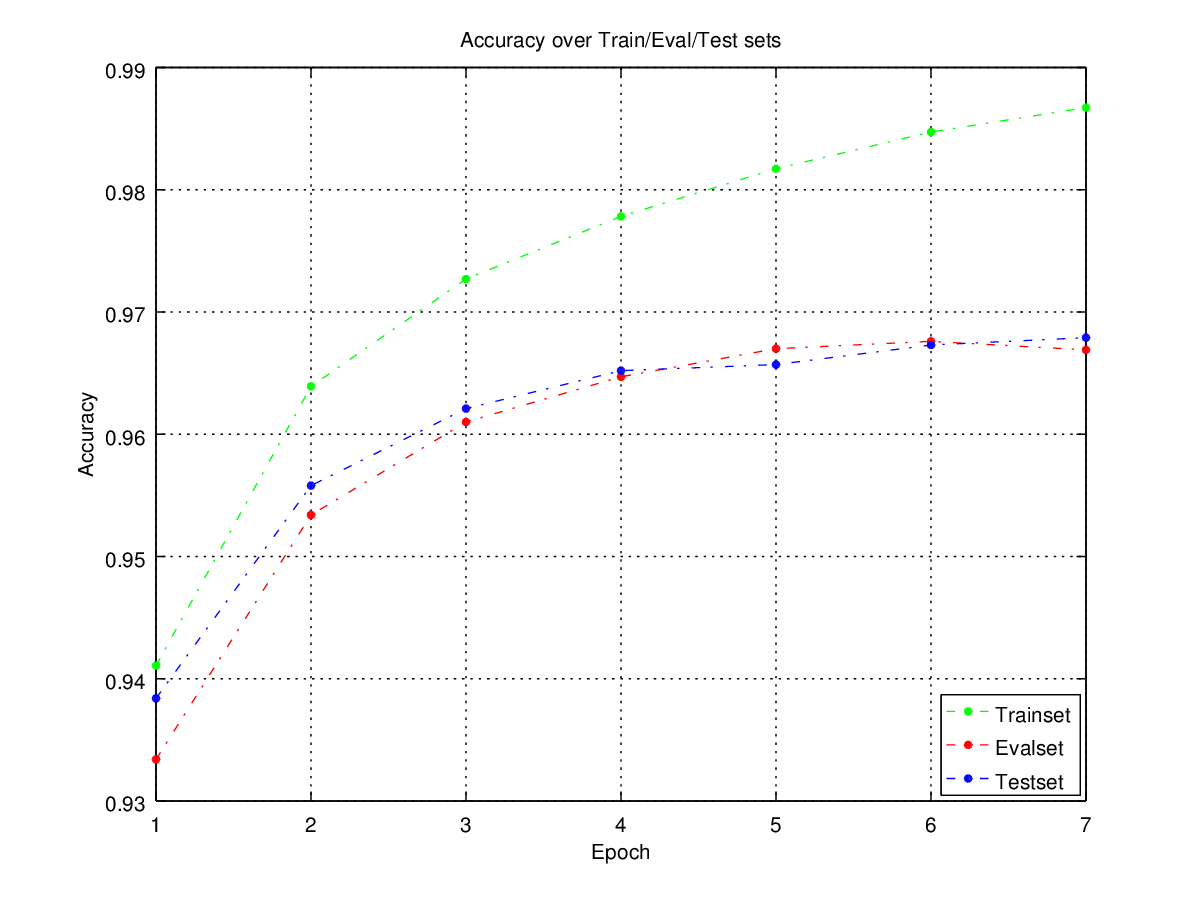
\includegraphics[width=.9\textwidth]{5_pca_acc}
\caption{مقدار دقت بروی داده\ های آموزشی، ارزیاب و تست در دوره\ های مختلف بعد از کاهش بعد}\label{fig:section_e_pca_acc}
\end{figure}
\begin{figure}[t!]
\centering
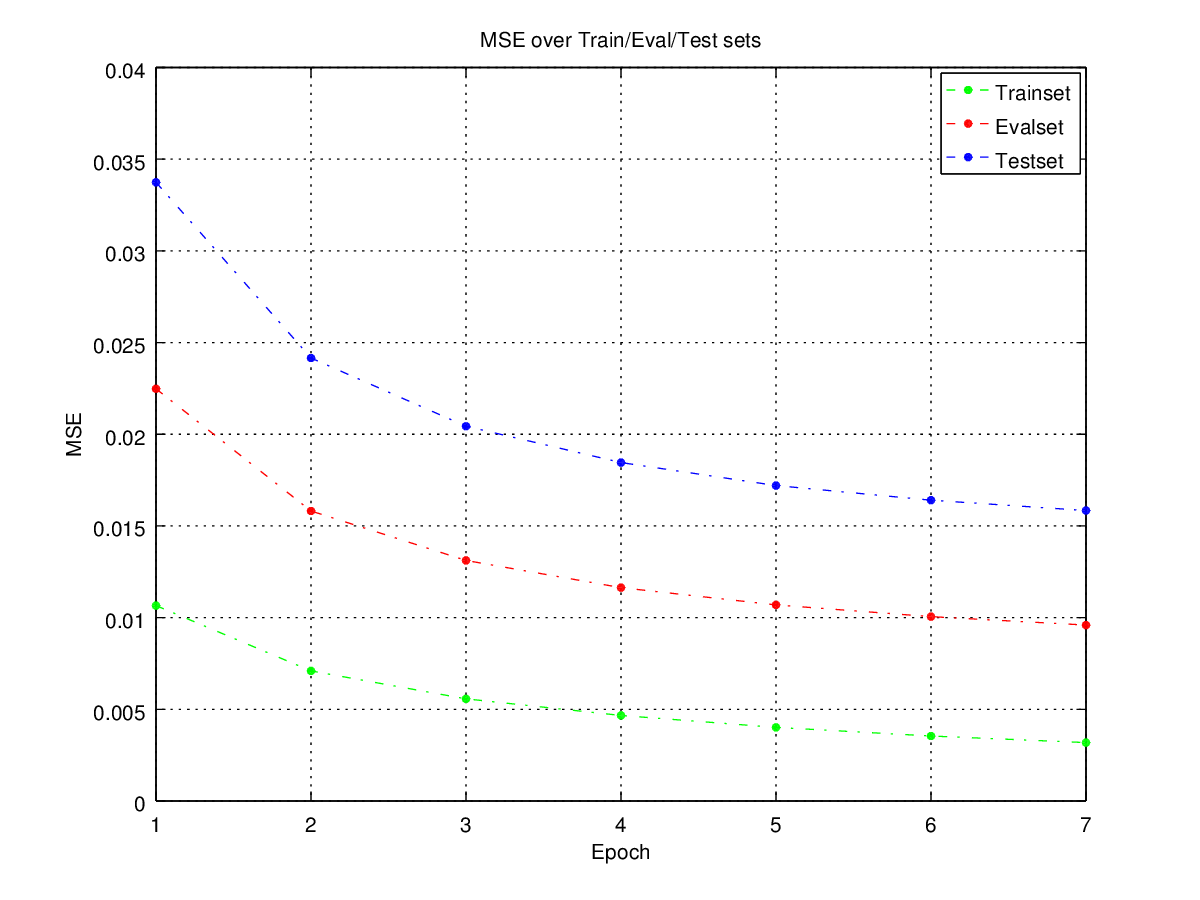
\includegraphics[width=.9\textwidth]{5_pca_mse}
\caption{مقدار میانگین \مسی خروجی\ های شبکه بروی داده\ های آموزشی، ارزیاب و تست در دوره\ های مختلف بعد از کاهش بعد}\label{fig:section_e_pca_mse}
\end{figure}
در شکل
\ref{fig:section_e_pca_diff_acc}
میزان اختلاف دقت قسمت\ های الف با داده\ های کاهش بعد یافته و یادگیری به روش دسته\ های کوچک آمده است. همان\ طور که می\ بینیم اختلاف چشم\ گیری بین دقت\ های قسمت الف و این قسمت وجود دارد و سرعت اجرا ۴۰ برابر کمتر از سرعت اجرای شبکه بروی داده\ های آموزشی کاهش\ بعد یافته می\ باشد. همان\ طور که در شکل
\ref{fig:section_e_pca_acc}
مشاهده می\ شود همانند قسمت الف جهش\ های ناگهانی در دقت در دوره\ های مختلف مشاهده نمی\ شود و دقت به صورت ملایم تغییر می\ کند. همین مساله برای شکل
\ref{fig:section_e_pca_mse}
نیز مشاهده\ ی می\ شود که مقادیر \مسی با ملایمت در طی زمان رو به کاهش\ اند. در شکل
\ref{fig:section_e_all_acc}
{\small
از بین دقت\ های قسمت\ های الف و ج و د، قسمت\ های  الف و ب تقریبا با یک دقت شروع کردند و قسمت د کمترین دقت را در انتهای کار داشت ولی درنهایت قسمت د بعد از نزدیک به ۶ دوره دقتش و از بقیه بیشتر شد}.
\newpage
\begin{figure}
\centering
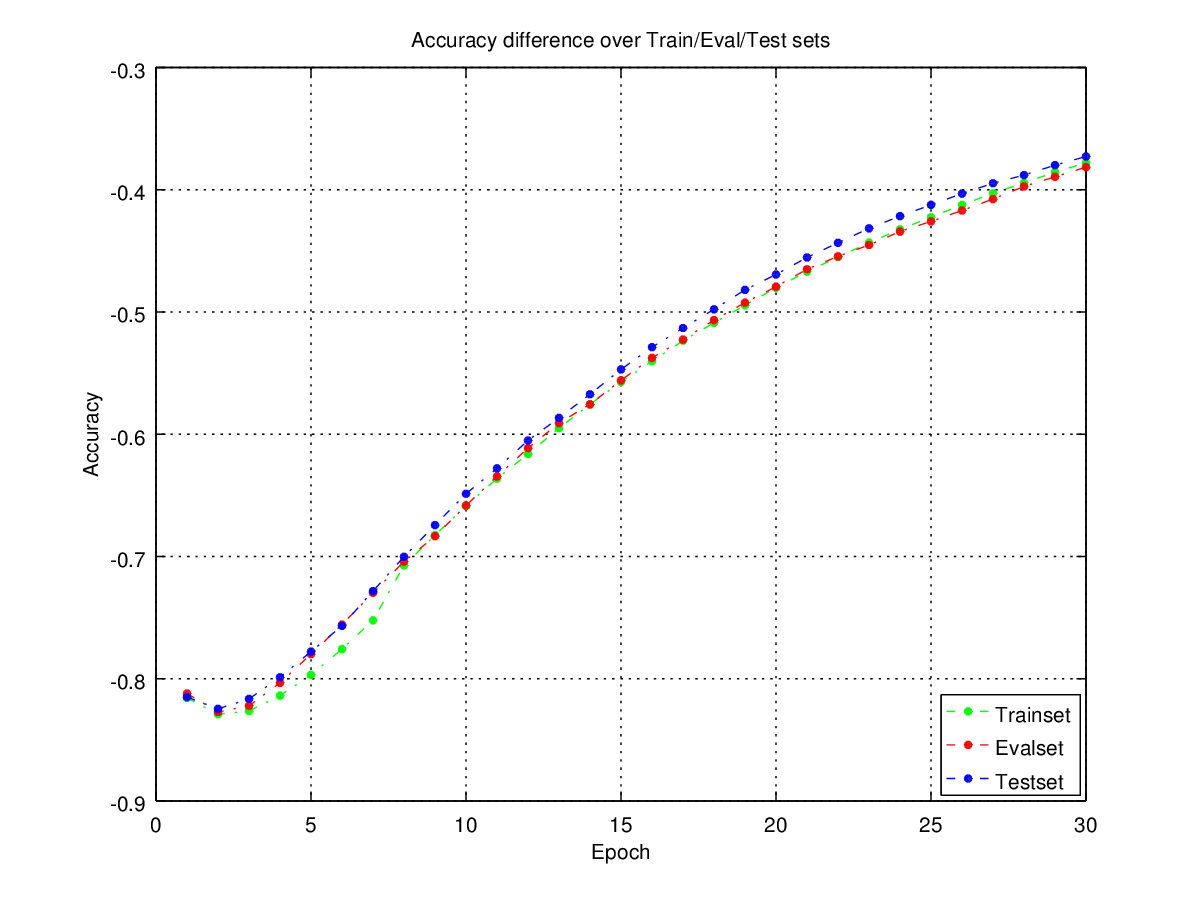
\includegraphics[width=.85\textwidth]{5_pca_diff_acc}
\caption{مقدار اختلاف دقت قسمت الف با دقت بدست آمده در شبکه\ ی آموزش دیده با استفاده از داده\ های کاهش بعد یافته در دوره\ های مختلف}\label{fig:section_e_pca_diff_acc}
\end{figure}
\begin{figure}
\centering
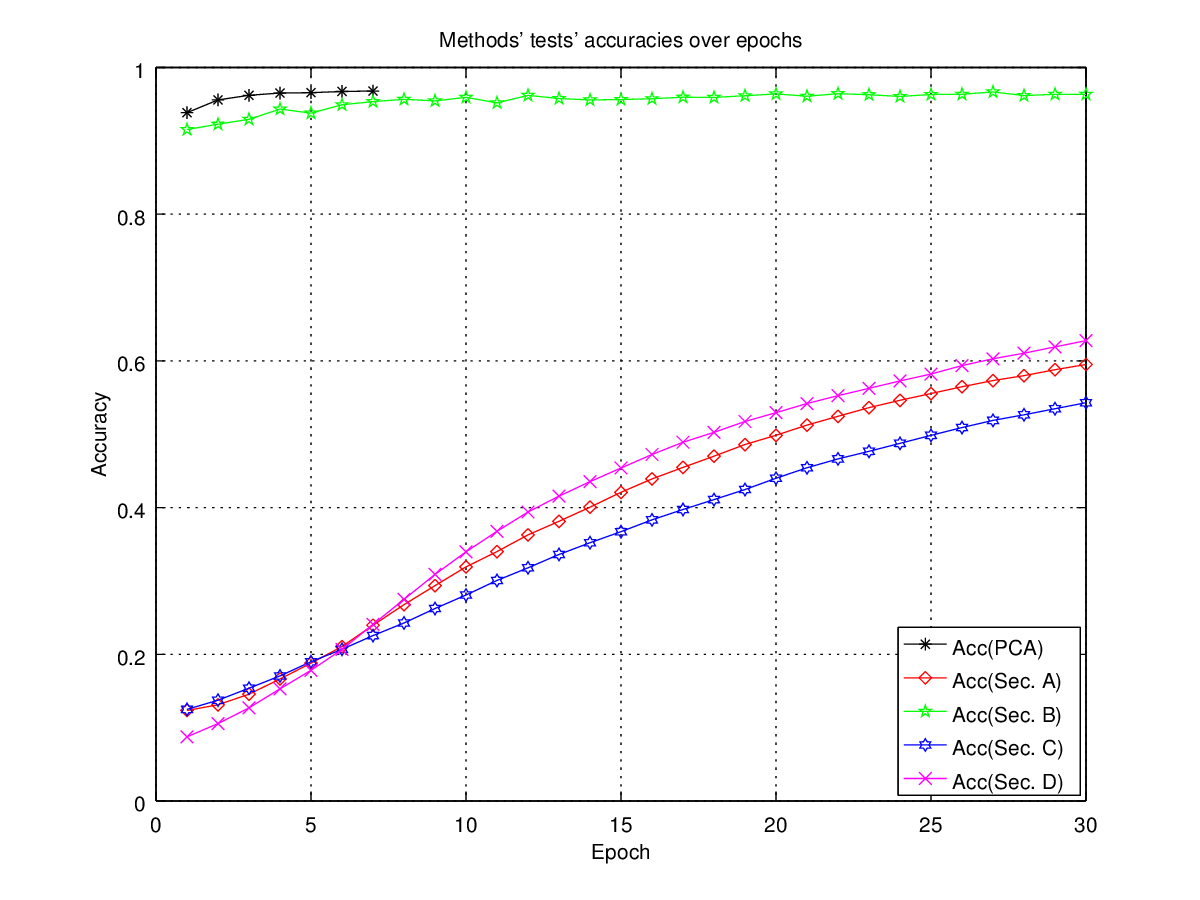
\includegraphics[width=.9\textwidth]{5_all_acc}
\caption{میزان دقت\ های قسمت مختلف در یک نگاه -- همان\ طور که می\ بینیم شبکه\ ای که بروی داده\ های کاهش بعد آموزش دیده با تعداد دوره\ های کمتر به دقتی رسید قسمت ب که از بین قسمت\ های فوق حداکثر دقت را داشت در انتهای کار خود به آن دقت نرسید(چند صدم با هم اختلاف دارند!!) و زودتر از موعد خاتمه پیدا کرد. }\label{fig:section_e_all_acc}
\end{figure}
\قسمت{نتیجه\ گیری و جمع\ بندی}
ما در این تکلیف به پیاده\ سازی الگوریتم \بپ پرداختیم و الگوریتم نوشته شده را بروی داده\ های \منست اجرا کرده و آزمودیم. در قسمت\ های مختلف این گزارش به بررسی نتایج اجرای الگوریتم با شیوه\ های مختلف پرداختیم. همان\ طور که گفته شد دقت در یادگیری به صورت دسته\ ای دارای افت\ وخیز ناگهانی نمی\ باشد و در آزمایشات ما به صورت ملایم در طی دوره\ ها رو افزایش بود ولی میزان این افزایش بسیار کم بود بگونه\ ای که بعد از ۶ ساعت آموزش به دقتی در حدود ۵۹٪ رسید. در قسمت ب مشاهده کردیم که دارای دقت بیشتری نسبت به دیگر قسمت\ ها داشت ولی در طی ۳۰ دوره\ ی معین شده هیچ یک از شروط توقف زودهنگام خود را ارضا نکرد و مانند دیگر قسمت\ ها بعد ۳۰ دوره به آموزش خاتمه داد و همچنین نسبت به بقیه مدت زیادی برای آموزش نیاز داشت(نزدیک به ۱۵ ساعت!!) و از طرف دیگر افت\ وخیزهای زیادی در میزان دقتش در دوره\ های مختلف مشاهده می\ شد. در قسمت ج نیز مشاهده کردیم که استفاده\ ی مومنتم باعث اینرسی در بروزرسانی وزن\ ها شد در نتیجه دقتش در مقایسه با قسمت الف با ملایمت بیشتری افزایش یافت و در نهایت دقتی کمتر از قسمت الف بدست آورد. در قسمت ج نیز مشاهده کردیم که دقت بروی داده\ های ارزیابی و تست به مقداری جزیی بیشتر از قسمت الف شد.
به عنوان ایده جهت افزایش دقت و سرعت همگرایی در قسمت آخر گزارش آمدیم داده\ ها را کاهش بعد دادیم و از ۷۸۴ بعد به ۱۰۰ بعد کاهش دادیم که این کاهش بعد به طرز چشم\ گیری در سرعت همگرایی و همچنین سرعت اجرای الگوریتم تاثیر گذاشت -- حدود ۵۰ برابر سرعت اجرایی، ۶ برابر حافظه\ ی مصرفی و ۴ برابر سرعت همگرایی بهتر شدند.
\end{document}
